%        File: fa18.tex
%     Created: Fri Dec 21 04:00 PM 2018 C
% Last Change: Fri Dec 21 04:00 PM 2018 C
%
\documentclass[a4paper]{article}
\usepackage{preamble}
\usepackage{374_preamble}
\usepackage{graphicx}
\graphicspath{./pictures}
\begin{document}

\tableofcontents
\section{Opening Remarks}


This is a progress report. \\

This report discusses work on a framework that allows home appliance users to subscribe their smart electronic appliances  to be activated at ``optimal times'' (we define ``optimal'' times in the background). \\

\section{Background Phenomena (and some buzzwords)}

\subsection{IoT}
IoT (Internet of Things) refers to the notion that everyday objects can be interacted with intelligiently over a network. This project is an IoT project, because we want to enable home appliances to turn on at ``optimal'' times.

\subsection{Serverless Computing}
Serverless computing describes the development of software and services in which maintenance of a server has been relegated to a third party. This project uses severless computing, becausethe transmission of data to home appliances takes place through a data pipeline. This pipeline is architected using components from serverless platforms, in particular AWS (Amazon Web Services).

\subsection{Varying Retail Price of Electricity}
Retail electricity rates in the United States vary over time and space, because electricity is a good subject to supply and demand. This causes retail rates to fall below their average price at times. For example, in the early morning, when electrical supply tends to ``outstrip'' demand for it, rates tend to be cheap. An example of price progression is shown, below, in a plot that traces the history of average hourly prices over different times of the day on May 25th, 2017.

    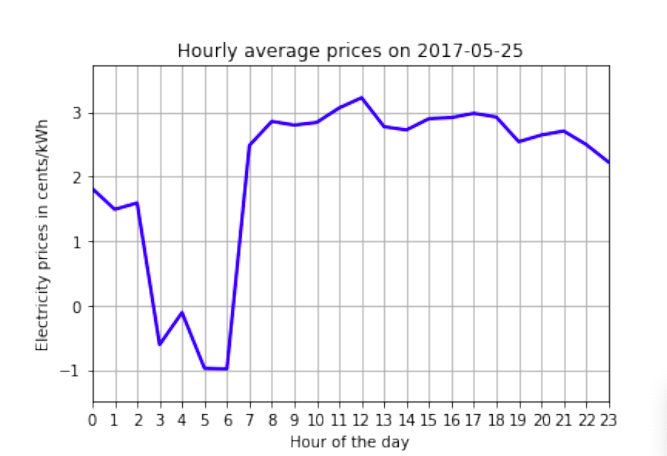
\includegraphics[width=0.7\paperwidth,height=0.7\paperheight,keepaspectratio]{../pictures/average_hourly_prices}

This plot hides one fact: that while price varies over time, they remain constant within an hour. This is significant, because it allows us to exercise the reasonable assumption that an appliance takes less than an hour to run. Let us formalize this a bit:
First, let us identify hours from the beginning of a day (ie 12:00 AM) to the day's end in terms of intervals like $(0,1], (1,2] \dots (n, n+1]$ (here, we let the intervals be right continuous). Under this identification, $(0,1]$ maps to $(12:00 \text{AM}, 1:00\text{AM}]$, $(1,2]$ maps to $(1:00 \text{AM}, 2:00\text{AM}]$ and so forth. Thus, if we want a device that runs for time $T$ to fall within an hour $(n, n+1]$, then the device must be made to run in the interval $(n, n+1 -T)$ or else fall over the interval. As a consequence, the ``optimal'' activation time to turn on an appliance running for time $T$ is during an interval $(n, n+1 - T]$, where the price over the hour $(n, n+1]$ is cheaper than during all other hours. It is the present work of Professor Richard Sowers and a graduate student, Rachneet Kaur, to create an algorithm that identifies this optimal time. This project (my thesis) accepts this algorithm as a black box.

\newpage


\section{Thesis Summary (Planned Intellectual Contribution)} 
A thesis ideally expands upon or redistills known findings of an intellectual field in a more revealing form. I hope to redistill existing technologies in IOT, serverless computing and machine learning in the form of a software framework. To my knowledge, there is no framework like the one I intend to create: \\

This framework allows home appliance users to subscribe their smart\footnote{I assume that the appliance already has an imbedded controller that can turn on the appliance after receiving an authenticated post request} electronic
appliances  to be activated at ``optimal times.'' An optimal time is defined in more detail in the background section. \footnote{Informally, an optimal time is a point in time beginning a time interval over which it is cheapest for a home user to run an appliance. This time interval falls between 11 PM to 5 AM.} \\

Concretely, this framework is a data pipeline and front end interface. The front end consists of a chat-bot, in particular an Amazon Alexa, and a registration website. A user must take two actions to subscribe an appliance to the framework. A user must first register appropriate credentials needed to turn on their appliance through the registration website; a user must then communicate her intent to turn on her appliance to Alexa using a verbal command. Most importantly, a user must indicate whether her appliance should activate now or at a later, optimal time before 5AM the following day. If she postpones activation, then an algorithm being developed by Professor Richard Sowers and his graduate student determines a later, optimal time; the appliance then runs at this time.

After creating this framework, I will address these questions:

\begin{outline}
    \1 Does this service scale well when used with many clients? What are the
    results from a simulation involving many clients?
    \2 For example, can the service choose an optimal activation point for each client, such
    that the time required to choose the optimal point does not vary too much over clients?
    \2 At present, shortly after deciding upon the optimal activation time, there is a small
    window separating the time of decision and the time an appliance can be last run \footnote{We make the simplification that appliances can be only activated at times such that they entirely run within an hour. This allows us to define, as a consequence, a final time when an appliance can be activated.}. If many clients use this framework, can they all have their appliances turned on within this window, or will system stress lead some clients to fall outside the window?
    \1 Does this service actually save money when physically implemented? Can we, as service providers, make the service profitable given that the serverless infrastructure is itself costly?
    \1 If time permits: If such a service begins to be used en masse, what
    outlook does the profitability of it have? Is there still a profit that can be made?
\end{outline}


\section{Progress}
I have worked on this project for, at the time of writing, a little over $3.5$ months. I will explain what I did on a month-by-month basis.

\subsection{September}
This project uses AWS. In particular, we use the AWS products called Lambda, DynamoDB, S3 and Cloudwatch. We primarily program in javascript using the node runtime environment. A controller imbedded into a dishwasher uses an IoT product and framework called Particle. During September, I learned how to use all of these tools.

\subsection{October}
Previous batches of students have already made an architecture (although, as future work explains, this architecture is nowhere near the state necessary for my proposed framework to function). This architecture had been stale for eight months prior to my entry into this project. With the help of a team-mate working on this project for independent study, I revived the existing infrastructure. Concretely, I made necessary modifications to the code base in order to use a previously developed functionality. This functionality is the ability to immediately turn on a single device through the Alexa interface.

After ``reviving'' the infrastructure, with the help of a teammate, I added functionality to allow an additional device (belonging to the same user owning the dishwasher) to be turned on immediately through an Alexa. We were previously only capable of turning on one device.

\subsection{November and December}
Working with a teammate closely in October, I observed that our work pattern was inefficient. He would write code, that I would write over, that he would write over and so forth. This took place, because we used the same space on the online AWS GUI (capable of hosting only one file) to write tests. This poor development practice prompted me to introduce ``devops'' tools into our workflow. These tools added not only local testing capabilities but introduced other workflow tools, which I explain below:

\begin{outline}
    \1 A core unit of computation in AWS is known as a Lambda function. A lambda function executes code in an somewhat customizable environment. It can be trigerred by AWS units and trigger other AWS units.
    \1 I added unit tests to several key functions, including those that are immediately invoked when Alexa parses user utterances, those invoked to turn on the particle remotely and the ``controller'' function which receives calls from one function in order to call other functions. \\
    \2 Using these tests, I detected bugs in the existing infrastructure. Some of these bugs were patched; some still remain to be patched.
    \1 I wrote a script that allows a user to remotely upload code to a Lambda function, to test an already uploaded Lambda function and to version an already uploaded Lambda function.
    \2 Using this script, I could more quickly deploy code from my local repository to the AWS repository. Everything has, as a consequence, become workable from my local machine; I no longer need to access the AWS GUI to run tests or invoke code.
    \1 Infrastructure as code refers to the collection of domain specific languages and tools that allow one to specify the structure of an architecture in code. With infrastructure as code (IAC), one can then deploy an expressed architecture through code.
    \1 I configured an infrastructure as code software to allow my team to not simply deploy an individual function's local code to AWS but to deploy a segment of our architecture to AWS.
    \2 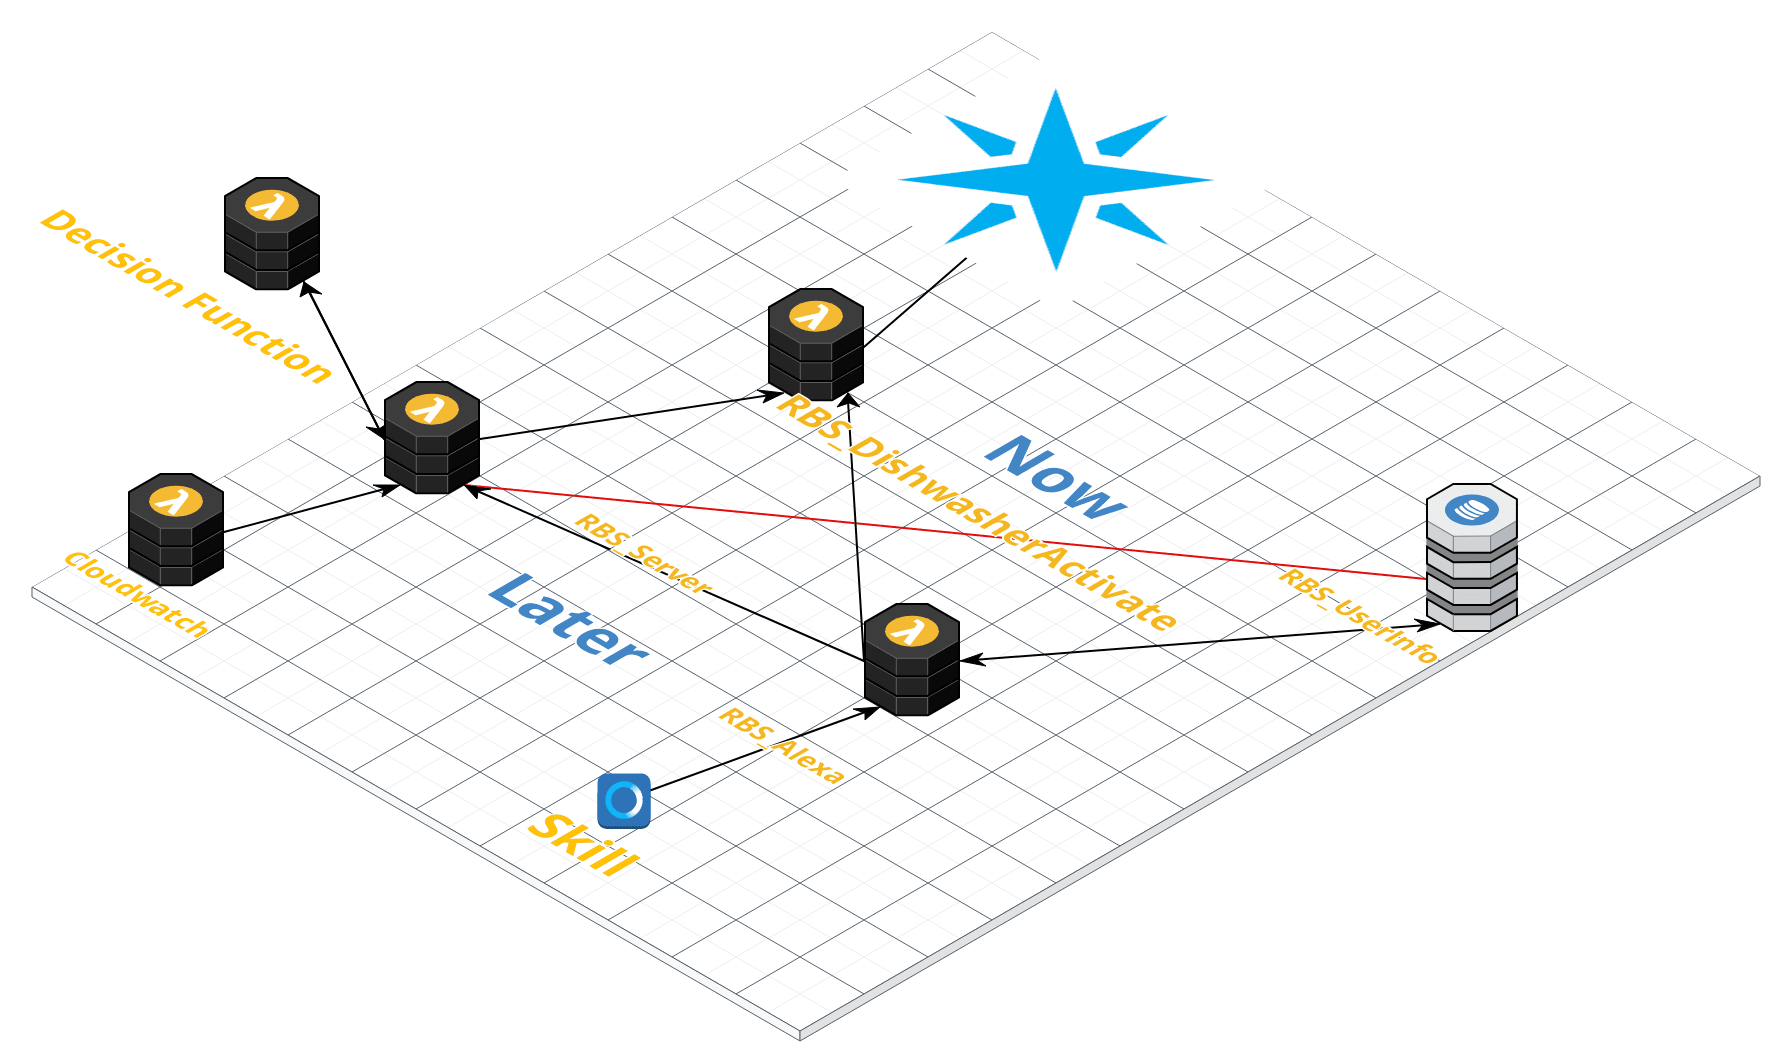
\includegraphics[width=0.7\paperwidth,height=0.7\paperheight,keepaspectratio]{../pictures/architecture}
    \2 Concretely, we can deploy the front end, which consists of the Alexa skill icon above, the function named RBS\_Alexa and the database named RBS\_userinfo.
\end{outline}

\section{Future Work}
Molding the infrastructure to become the framework I proposed will reqire several \textit{design choices and developments} and some other dev-ops work.
\begin{outline}
    \1 \textit{More DevOps:}
    \2  Devise a way of remotely 
    verifying whether the infrastructure caused the device to switch on at an ``optimal'' time.
    \2  Devise a way to simulate many clients using this service and to test the ability of the service to handle their requests.
    \1 \textit{Design:}
    \1  Expand the range of utterances the Alexa front end can use.
    \1  Make the dialogues interactive.
    \1  Change the database schema to remove duplication of appliance information.
    \1 Design a website that allows users to add their credentials.
    \1 The algorithm that chooses an optimal activation time first creates a prediction function that, in turn, chooses the activation time. This prediction function is expensive to compute and is useable by multiple clients. Thus, a way must be designed for the decision function to be shared.
    \1 If multiple clients express an intent to activate their appliance at a later, optimal time, then some function must be developed that allows the decison algorithm to be run in parallel for each of these users (at present, the architecture can only conceivably support iterative use of the decision algorithm).
    \end{outline}
\subsection{Relationship between Current Progress and Future Work}
In short, my work up to date has been an investment. The return on this investment will be shorter development time for the design of the framework than I would have otherwise needed. More directly, some of the tests I have written have already identified some bugs with the existing infrastructure that need to be redressed.


\end{document}




